\documentclass{article}

\usepackage[utf8]{inputenc}

\usepackage{hyperref}
\usepackage{nicefrac}
\usepackage{amssymb, amsmath, amsfonts}
\usepackage{amsthm}
\usepackage{tikz}
\usetikzlibrary{matrix,shapes,arrows, calc, intersections}
\usepackage{pgfplots}
\usepgfplotslibrary{groupplots}
\usepackage[a4paper, margin=1in]{geometry}

\newtheorem{proposition}{Proposition}
\newtheorem{theorem}{Theorem}
\newtheorem{definition}{Definition}
\newtheorem{lemma}{Lemma}
\newtheorem{conjecture}{Conjecture}
\newtheorem{corollary}{Corollary}
\newtheorem{remark}{Remark}
\newtheorem{assumption}{Assumption}

\newlength\figureheight
\newlength\figurewidth
\setlength\figureheight{12cm}
\setlength\figurewidth{14cm}

\newcommand{\tikzdir}[1]{tikz/#1.tikz}
\newcommand{\inputtikz}[1]{\input{\tikzdir{#1}}}

\DeclareMathOperator*{\argmin}{arg\; min}     % argmin
\DeclareMathOperator*{\argmax}{arg\; max}     % argmax
\DeclareMathOperator*{\tr}{tr}     % trace
\DeclareMathOperator{\Cov}{Cov}
\DeclareMathOperator{\logdet}{log\;det}

\title{EE8087 Living with Mathematics\\Lecture 2: Additional Notes}
\date{}
\begin{document} \maketitle
\begin{enumerate}
\item [Page 3:] How to find the maximum value of $\cos\alpha+\mu\sin\alpha$.

  \begin{figure}[ht]
    \centering
    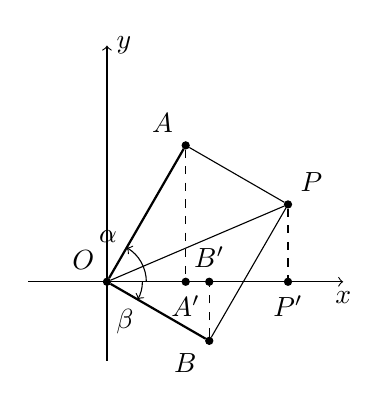
\begin{tikzpicture}[scale=0.5]
      \tikzset{mark coordinate/.style={inner sep=0pt,
          outer sep=0pt,
          minimum size=3pt,
          fill=#1,
          circle}
      }
      \draw [->] (-2,0)--(6,0);
      \node [anchor=north] at (6,0) {$x$};
      \draw [->] (0,-2)--(0,6);
      \node [anchor=west] at (0,6) {$y$};
      
      \node [mark coordinate=black,label=135:$O$] (O) at (0,0) {};
      \node [mark coordinate=black,label=135:$A$] (A) at (60:4) {};
      \node [mark coordinate=black,label=270:$A'$] (Ap) at (A|-O) {};
      \draw [thick] (O)--(A);

      \draw [dashed] (A)--(Ap);

      \node [mark coordinate=black,label=225:$B$] (B) at (-30:3) {};
      \node [mark coordinate=black,label=90:$B'$] (Bp) at (B|-O) {};
      \draw [thick] (O)--(B);
      \draw [dashed] (B)--(Bp);
      
      \node [mark coordinate=black,label=45:$P$] (P) at ($(A)+(B)$) {};
      \node [mark coordinate=black,label=270:$P'$] (Pp) at (P|-O) {};
      \draw [dashed] (P)--(Pp);

      \draw  (B)--(P);
      \draw  (A)--(P);
      \draw  (O)--(P);
      
      \draw [->](1,0) arc (0:60:1) node [anchor=-30] {$\alpha$};
      \draw [->](0.9,0) arc (0:-30:0.9) node [anchor=60]{$\beta$};
    \end{tikzpicture}
  \end{figure}

Assuming that $OA = 1$ and $OB = \mu$. Moreover, $OA$ are perpendicular to $OB$. 

Then we know $OA'= OA \times \cos\alpha = \cos \alpha$ and $OB' = OB \times \cos \beta = \mu \cos \beta$. Since $\alpha + \beta = 90^\circ$, $OB' = \mu \sin \alpha$. 

For the rectangle $OAPB$, we know that the projection $A'P' = OB'$ since $AP = OB$ and they are parallel. As a result,

\begin{align*}
  OP' = OA'+A'P' = OA' + OB' = \cos\alpha+\mu\sin\alpha.
\end{align*}

In order to maximize the projection $OP'$, we need to make $P$ on the $x$-axis. This requires that $\alpha = \angle AOP = \tan^{-1}\mu$, and the maximum $OP' = OP = \sqrt{1+\mu^2}$.

To understand this more, you can click on the following \href{https://www.desmos.com/calculator/0rbehs0dfw}{interactive example}.

\item[Page 27:] How to solve the differential equation $\nicefrac{dy}{dt} + y = x$ when $x = \sin(\omega t)$.
  
We will guess the solution is $y = A \sin(\omega t + \phi)$. If so, then the differential equation becomes
\begin{align*}
  \sin(\omega t) &= A \omega \cos(\omega t+\phi) + A \sin(\omega t + \phi)\\
&= (A \omega \cos \phi + A \sin \phi) \cos (\omega t) +  (-A \omega \sin \phi + A \cos \phi) \sin (\omega t).
\end{align*}
As a result, we need to find $A$ and $\phi$, such that
\begin{align*}
 A \omega \cos \phi + A \sin \phi& = 0,\\
-A \omega \sin \phi + A \cos \phi &=1.
\end{align*}
From the first equation, we know that $tan \phi = -\omega$, so $\phi = -\tan^{-1}\omega$ and $\sin \phi = -\nicefrac{\omega}{\sqrt{1+\omega^2}}$ and $\cos \phi = \nicefrac{1}{\sqrt{1+\omega^2}}$. Now use the second equation we can prove that $A = \nicefrac{1}{\sqrt{1+\omega^2}}$. Hence,
\begin{align*}
 y = \frac{1}{\sqrt{1+\omega^2}}\sin(\omega t - \tan^{-1}\omega) 
\end{align*}


\end{enumerate}

\end{document}
%%% Local Variables:
%%% TeX-command-default: "Latexmk"
%%% End:
